\documentclass{article}
\usepackage[utf8]{inputenc} % Allow utf-8 input
\usepackage[T1]{fontenc}    % Use 8-bit T1 fonts
\usepackage{graphicx}       % Required for inserting images
\usepackage{booktabs}       % Professional-quality tables
\usepackage{amsfonts}       % Blackboard math symbols
\usepackage{nicefrac}       % Compact symbols for 1/2, etc.
\usepackage{microtype}      % Microtypography
\usepackage[colorlinks=true, linkcolor=blue, citecolor=red, filecolor=magenta, urlcolor=cyan]{hyperref} % Hyperlinks
\usepackage{halloweenmath}
\usepackage{subcaption}
\usepackage{calrsfs}
\usepackage{listings}
\usepackage{authblk}
\usepackage{ragged2e}
\usepackage{amsmath}
\usepackage{amssymb}
\usepackage{color}
\usepackage{amsthm}
\usepackage{bm}
\usepackage{algorithm}
\usepackage{algpseudocode}
\usepackage{dsfont}
\usepackage{bbm}
\usepackage{enumitem}
\usepackage[dvipsnames]{xcolor}
\usepackage{geometry}
\usepackage{comment}
\usepackage{float}
\usepackage{booktabs}
\usepackage{titling}
\renewcommand\maketitlehooka{\null\mbox{}\vfill}
\renewcommand\maketitlehookd{\vfill\null}

% Define colors for Python syntax highlighting
\definecolor{pythonblue}{RGB}{0,0,255}
\definecolor{pythongreen}{RGB}{0,128,0}
\definecolor{pythonpurple}{RGB}{128,0,128}
\definecolor{pythongray}{RGB}{128,128,128}

\geometry{a4paper, margin=1in}

\setlength{\parindent}{0pt} % Remove paragraph indentation
\setlength{\parskip}{0.5em} % Add space between paragraphs

\renewcommand{\algorithmicrequire}{\textbf{Input:}}
\renewcommand{\algorithmicensure}{\textbf{Output:}}

\def\c{\boldsymbol{c}}
\def\ud{\underline}
\def\e{\varepsilon}
\def\R{{\mathbb{R}}}
\def\Q{\mathbb{Q}}
\def\Z{\mathcal{Z}}
\def\X{\mathcal{X}}
\def\Y{\mathcal{Y}}
\def\N{\mathbb{N}}
\def\II{{\rm I\kern-0.5exI}}
\def\III{{\rm I\kern-0.5exI\kern-0.5exI}}
\DeclareMathOperator{\grad}{grad}

% == Basic commands == %
\newcommand{\dotprod}[2]{\langle #1, #2 \rangle}
\newcommand{\abs}[1]{\lvert #1 \rvert}
\newcommand{\abss}[1]{\left\lvert #1 \right\rvert}
\newcommand{\norm}[1]{\lVert #1 \rVert}
\newcommand{\normm}[1]{\left\lVert #1 \right\rVert}
\newcommand{\set}[1]{\left\{\, #1 \,\right\}}
\newcommand{\bracket}[1]{\langle #1 \rangle}
\newcommand{\iif}{\Leftrightarrow}
\newcommand{\conv}{\star}

% Sets
\newcommand{\RR}{\mathbb{R}}
\newcommand{\CC}{\mathbb{C}}
\newcommand{\ZZ}{\mathbb{Z}}
\newcommand{\TT}{\mathbb{T}}
\newcommand{\PP}{\mathbb{P}}
\newcommand{\FF}{\mathbb{F}}
\newcommand{\VV}{\mathbb{V}}
\newcommand{\EE}{\mathbb{E}}
\newcommand{\M}{\mathcal{M}}
\newcommand{\Real}{\mathbf{R}}
\newcommand{\Integ}{\mathbf{Z}}
\newcommand{\RN}{\mathbf{R}^N}
\newcommand{\Rd}{\mathbf{R}^d}
\newcommand{\Rn}{\mathbf{R}^n}
\newcommand{\veps}{\varepsilon}
\newcommand{\F}{\mathcal{F}}
\newcommand{\E}{\mathbb{E}}
\newcommand{\I}{\mathcal{I}}
\newcommand{\T}{\mathcal{T}}
\newcommand{\cF}{\mathcal{F}}
\newcommand{\cFall}{\mathcal{F}_{\text{all}}}
\newcommand{\cB}{\mathcal{B}}
\newcommand{\cH}{\mathcal{H}}
\newcommand{\cU}{\mathcal{U}}
\newcommand{\cN}{\mathcal{N}}
\newcommand{\cT}{\mathcal{T}}
\newcommand{\cX}{\mathcal{X}}
\newcommand{\cY}{\mathcal{Y}}
\newcommand{\cZ}{\mathcal{Z}}
\newcommand{\eps}{\varepsilon}
\newcommand{\tx}{\tilde{x}}
\newcommand{\ty}{\tilde{y}}
\newcommand{\tz}{\tilde{z}}
\newcommand{\tA}{\tilde{A}}
\newcommand{\tR}{\tilde{R}}
\newcommand{\tmu}{\tilde{\mu}}
\newcommand{\1}{\mathbbm{1}}
\DeclareMathOperator{\essinf}{essinf}
\DeclareMathOperator{\esssup}{esssup}
\DeclareMathOperator{\supp}{supp}
\DeclareMathOperator{\PRL}{PRL}

% Colors
\newcommand{\red}{\color{red}}
\newcommand{\blue}{\color{blue}}
\newcommand{\nc}{\normalcolor}

\newtheorem{theorem}{Theorem}
\newtheorem{proposition}{Proposition}
\theoremstyle{definition}
\newtheorem{definition}{Definition}
\linespread{1.5}

\makeatletter
\newcommand*\bigcdot{\mathpalette\bigcdot@{.5}}
\newcommand*\bigcdot@[2]{\mathbin{\vcenter{\hbox{\scalebox{#2}{$\m@th#1\bullet$}}}}}
\makeatother

\begin{document}
\title{\textbf{
    Modeling and Forecasting Walmart Stock Prices: A Comparative Analysis of ARMA and ARCH Approaches
}}

\author{Shrivats Sudhir}
\date{December 16, 2023}

\begin{titlingpage}
\maketitle
\end{titlingpage}


\newpage
\pagenumbering{arabic} % Start normal page numbering
\section{Introduction}

Understanding stock price dynamics is crucial for informed investment decisions. This study models and forecasts Walmart Inc.'s (WMT) daily adjusted closing prices from \texttt{2020-01-01} to \texttt{2023-12-06} with the following objectives: (1) Compute log returns, (2) Find the optimal \texttt{ARIMA} and \texttt{GARCH} models to capture volatility clustering and conditional heteroskedasticity, (3) Fit an ensemble Validate models using AIC, BIC, and residual diagnostics, and (4) Generate a 10-step ahead forecast to provide actionable insights for investors and risk managers by modeling and forecasting stock price movements.

Let $P_t$ be the price of an asset at time $t$, then the log returns is defined as:
$$r_t = \text{log}\;P_t - \text{log}\;P_{t-1}$$

\begin{figure}[H]
\centering
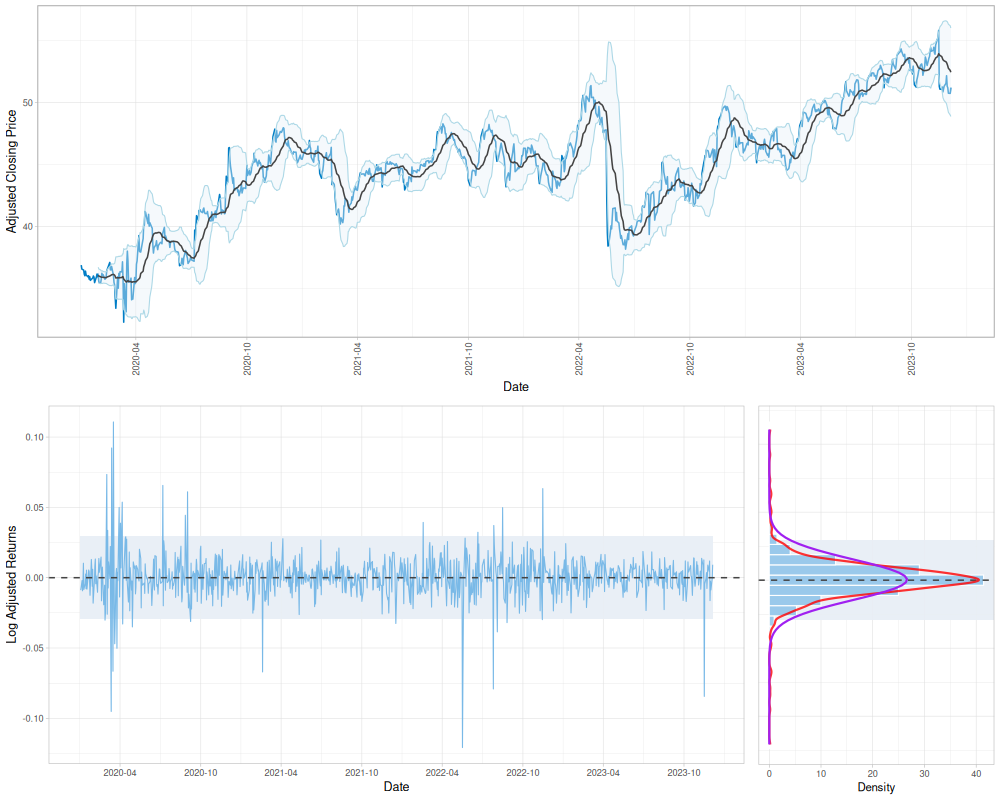
\includegraphics[width=1.0\textwidth]{Walmart_Stock_Analysis.png}
\caption{\small{\href{https://github.com/Stochastic1017/Walmart-Stock-Forecasting/blob/main/R/Plot_AdjClose_LogReturns.R}{Walmart Inc.'s adjusted closing prices with Bollinger Bands, log returns with a 95\% confidence interval, and a histogram of log returns with KDE and theoretical normal distribution.}}}
\label{fig:adjclose_adjreturns_plot}
\end{figure}

From Figure \ref{fig:adjclose_adjreturns_plot}, there seems to exist some volatility clusters that need to be addressed. Furthermore, the log return distribution seems to be Leptokurtic in nature, illustrating heavy tails and deviations from normality. We now proceed with rigorously testing for normality and stationarity.








\section{Fitting \texttt{ARIMA} Model}

The \texttt{forecast} package in R allows us to use \texttt{auto.arima} which automatically selects the best model based on AIC/BIC.

\begin{table}[H]
\centering
\begin{tabular}{l|r}
\hline
\textbf{Model}  & \textbf{ARIMA(0,0,1) with zero mean} \\
\hline
MA1 Coefficient & -0.0666 \\
Standard Error  & 0.0312 \\
$\sigma^2$      & 0.0002266 \\
\hline
Log-Likelihood  & 2694.43 \\
AIC             & -5384.85 \\
AICc            & -5384.84 \\
BIC             & -5375.1 \\
\hline
\end{tabular}
\caption{\small{\href{https://github.com/Stochastic1017/Walmart-Stock-Forecasting/blob/main/R/Fit_ARMA.R}{Summary of fitted ARMA model.}}}
\label{tab:arma_model_summary}
\end{table}

The fitted \texttt{ARIMA(0,0,1)} model for Walmart Inc.'s log returns is summarized in Table \ref{tab:arma_model_summary}, with a moving average coefficient of $-0.0666$ (standard error = $0.0312$), indicating weak short-term autocorrelation. The residual variance is estimated as $\sigma^2 = 0.0002266$, and model selection criteria, including AIC ($-5384.85$) and BIC ($-5375.1$), confirm its suitability.

In mathematical terms, we can write the \texttt{ARIMA} model as:
$$r_t = a_t - (-0.0666) \cdot a_{t-1}$$
where $a_t \sim N(0, 0.0312)$ and $\mathbb{E}[r_t] = 0$.


\section{Fitting \texttt{ARCH/GARCH} Models}

The \texttt{fGarch} library in R allows us to fit various \texttt{GARCH} models and compare performances between the them. For the purposes of keeping the models simple and explainable, the focus is on \texttt{GARCH}(1,0) and \texttt{GARCH}(1,1), using conditional distributions from \texttt{c("norm", "ged", "std", "snorm", "sged", "sstd")}.

\begin{table}[H]
\centering
\begin{minipage}[t]{0.48\textwidth} % Left table (Normality Tests)
\centering
\scriptsize % Reduce font size
\begin{tabular}{l|r}
\hline
\textbf{Model}  & \texttt{GARCH(1,0), cond.dist="std"} \\
\hline
mu & 6.090e-04\\
omega & 1.505e-04\\
alpha1 & 2.988e-01\\
shape & 3.436e+00\\
\hline
Log-Likelihood  & 2908.097 \\
AIC             & -5.987829 \\
BIC             & -5.967716 \\
SIC             & -5.987863\\
HQIC            & -5.980173\\
\hline
\end{tabular}
\end{minipage}
\hfill
\begin{minipage}[t]{0.48\textwidth} % Right table (Stationarity Tests)
\centering
\scriptsize % Reduce font size
\begin{tabular}{l|r}
\hline
\textbf{Model}  & \texttt{GARCH(1,1), cond.dist="std"} \\
\hline
mu              & 5.220e-04\\
omega           & 1.560e-05\\
alpha1          & 1.291e-01\\
beta1           & 7.905e-01\\
shape           & 4.062e+00\\
\hline
Log-Likelihood  & 2929.534 \\
AIC             & -6.029967 \\
BIC             & -6.004826 \\
SIC             & -6.030020\\
HQIC            & -6.020398\\
\hline
\end{tabular}
\end{minipage}
\caption{\small{\href{https://github.com/Stochastic1017/Walmart-Stock-Forecasting/blob/main/R/Fit_ARCH_GARCH.R}{Summary of fitted ARCH and GARCH model.}}}
\label{tab:arch_garch_model_summary}
\end{table}

Table \ref{tab:arch_garch_model_summary} summarizes the fitted \texttt{GARCH(1,0)} and \texttt{GARCH(1,1)} models using a Student-t conditional distribution, which among all other conditional distribution options best maximizes log-likelihood with reasonable AIC, BIC, SIC, HQIC values. Although \texttt{GARCH(1,0)} achieves slightly lower AIC (-5.99 vs. -6.03) and BIC (-5.97 vs. -6.00), indicating a marginally better balance between model fit and complexity, we find that \texttt{GARCH(1,1)} achieves a higher log-likelihood (2929.534 vs. 2908.097) and captures long-term volatility persistence through the additional $\beta_1$ parameter, which is crucial for financial time series exhibiting volatility clustering. Therefore, we prefer \texttt{GARCH(1,1)} over \texttt{GARCH(1,0)}.

In mathematical terms, we can write the \texttt{GARCH(1,1)} model as:
$$a_t = \sigma_t \epsilon_t, \quad \sigma^2_t = (\text{1.560e-05}) + (\text{1.291e-01})a^2_{t-1} + (\text{7.905e-01})\sigma^2_{t-1}$$
where $\epsilon_t \sim \text{std}(0,1)$ with shape parameter 4.0624. The relatively large value of $\beta_1$ (0.7905) relative to $\alpha_1$ (0.1291) reflects the long memory in volatility, which is consistent with financial time series exhibiting volatility clustering.






\section{Fitting Ensemble $\texttt{ARIMA(0,0,1)}+\texttt{GARCH(1,1)}$ Model}

A preliminary $\texttt{ARIMA(0,0,1)}+\texttt{GARCH(1,1)}$ model with a Student-t conditional distribution is fitted to the log returns to capture volatility clustering and heavy tails. We iteratively detect and remove influential points (standardized residuals exceeding a threshold of $\pm 3$) by fitting until the process continues until no new influential points are identified, or the changes in residual diagnostics become negligible.

\begin{table}[H]
\centering
\begin{tabular}{l|r}
\hline
\textbf{Model}  & \texttt{ARIMA(0,0,1) + GARCH(1,1)} \\
\hline
mu & 4.9198e-04 \\
omega  & 6.3505e-06 \\
alpha1      & 1.0224e-01 \\
beta1 & 8.5001e-01\\
shape & 1.0000e+01\\
\hline
Log-Likelihood  & 2972.232\\
AIC             & -6.246803\\
BIC             & -6.221243\\
SIC             & -6.246858\\
HQIC            & -6.237065\\
\hline
\end{tabular}
\caption{\small{\href{https://github.com/Stochastic1017/Walmart-Stock-Forecasting/blob/main/R/Fit_ARMA_and_GARCH.R}{Summary of fitted ARMA(0,0,1)+GARCH(1,1) model.}}}
\label{tab:arma_garch_model_summary}
\end{table}

From Table \ref{tab:arma_garch_model_summary}, we can see that there is a substantial increase in log-likelihood compared to individual \texttt{GARCH(1,1)} or \texttt{ARIMA(0,0,1)} models, with only slight increase in AIC and BIC. Furthermore, the statistically significant $\beta_1$ value (0.8501) indicates strong long-term persistence in volatility, while the moderate statistically significant $\alpha_1$ value (0.1022) captures short-term shocks effectively.








\section{Residual Diagnostics}

Figure \ref{fig:residual_diagnostics} show that the fitted ensemble model is satisfactory. The residuals over time are random around zero, the histogram aligns with a normal distribution, the Q-Q plot shows minimal deviation from normality, and the ACF plots confirm no significant autocorrelation in residuals, squared residuals, or absolute residuals, indicating no remaining structure or volatility clustering.



\begin{figure}[H]
\centering
\begin{subfigure}{\textwidth}
    \centering
    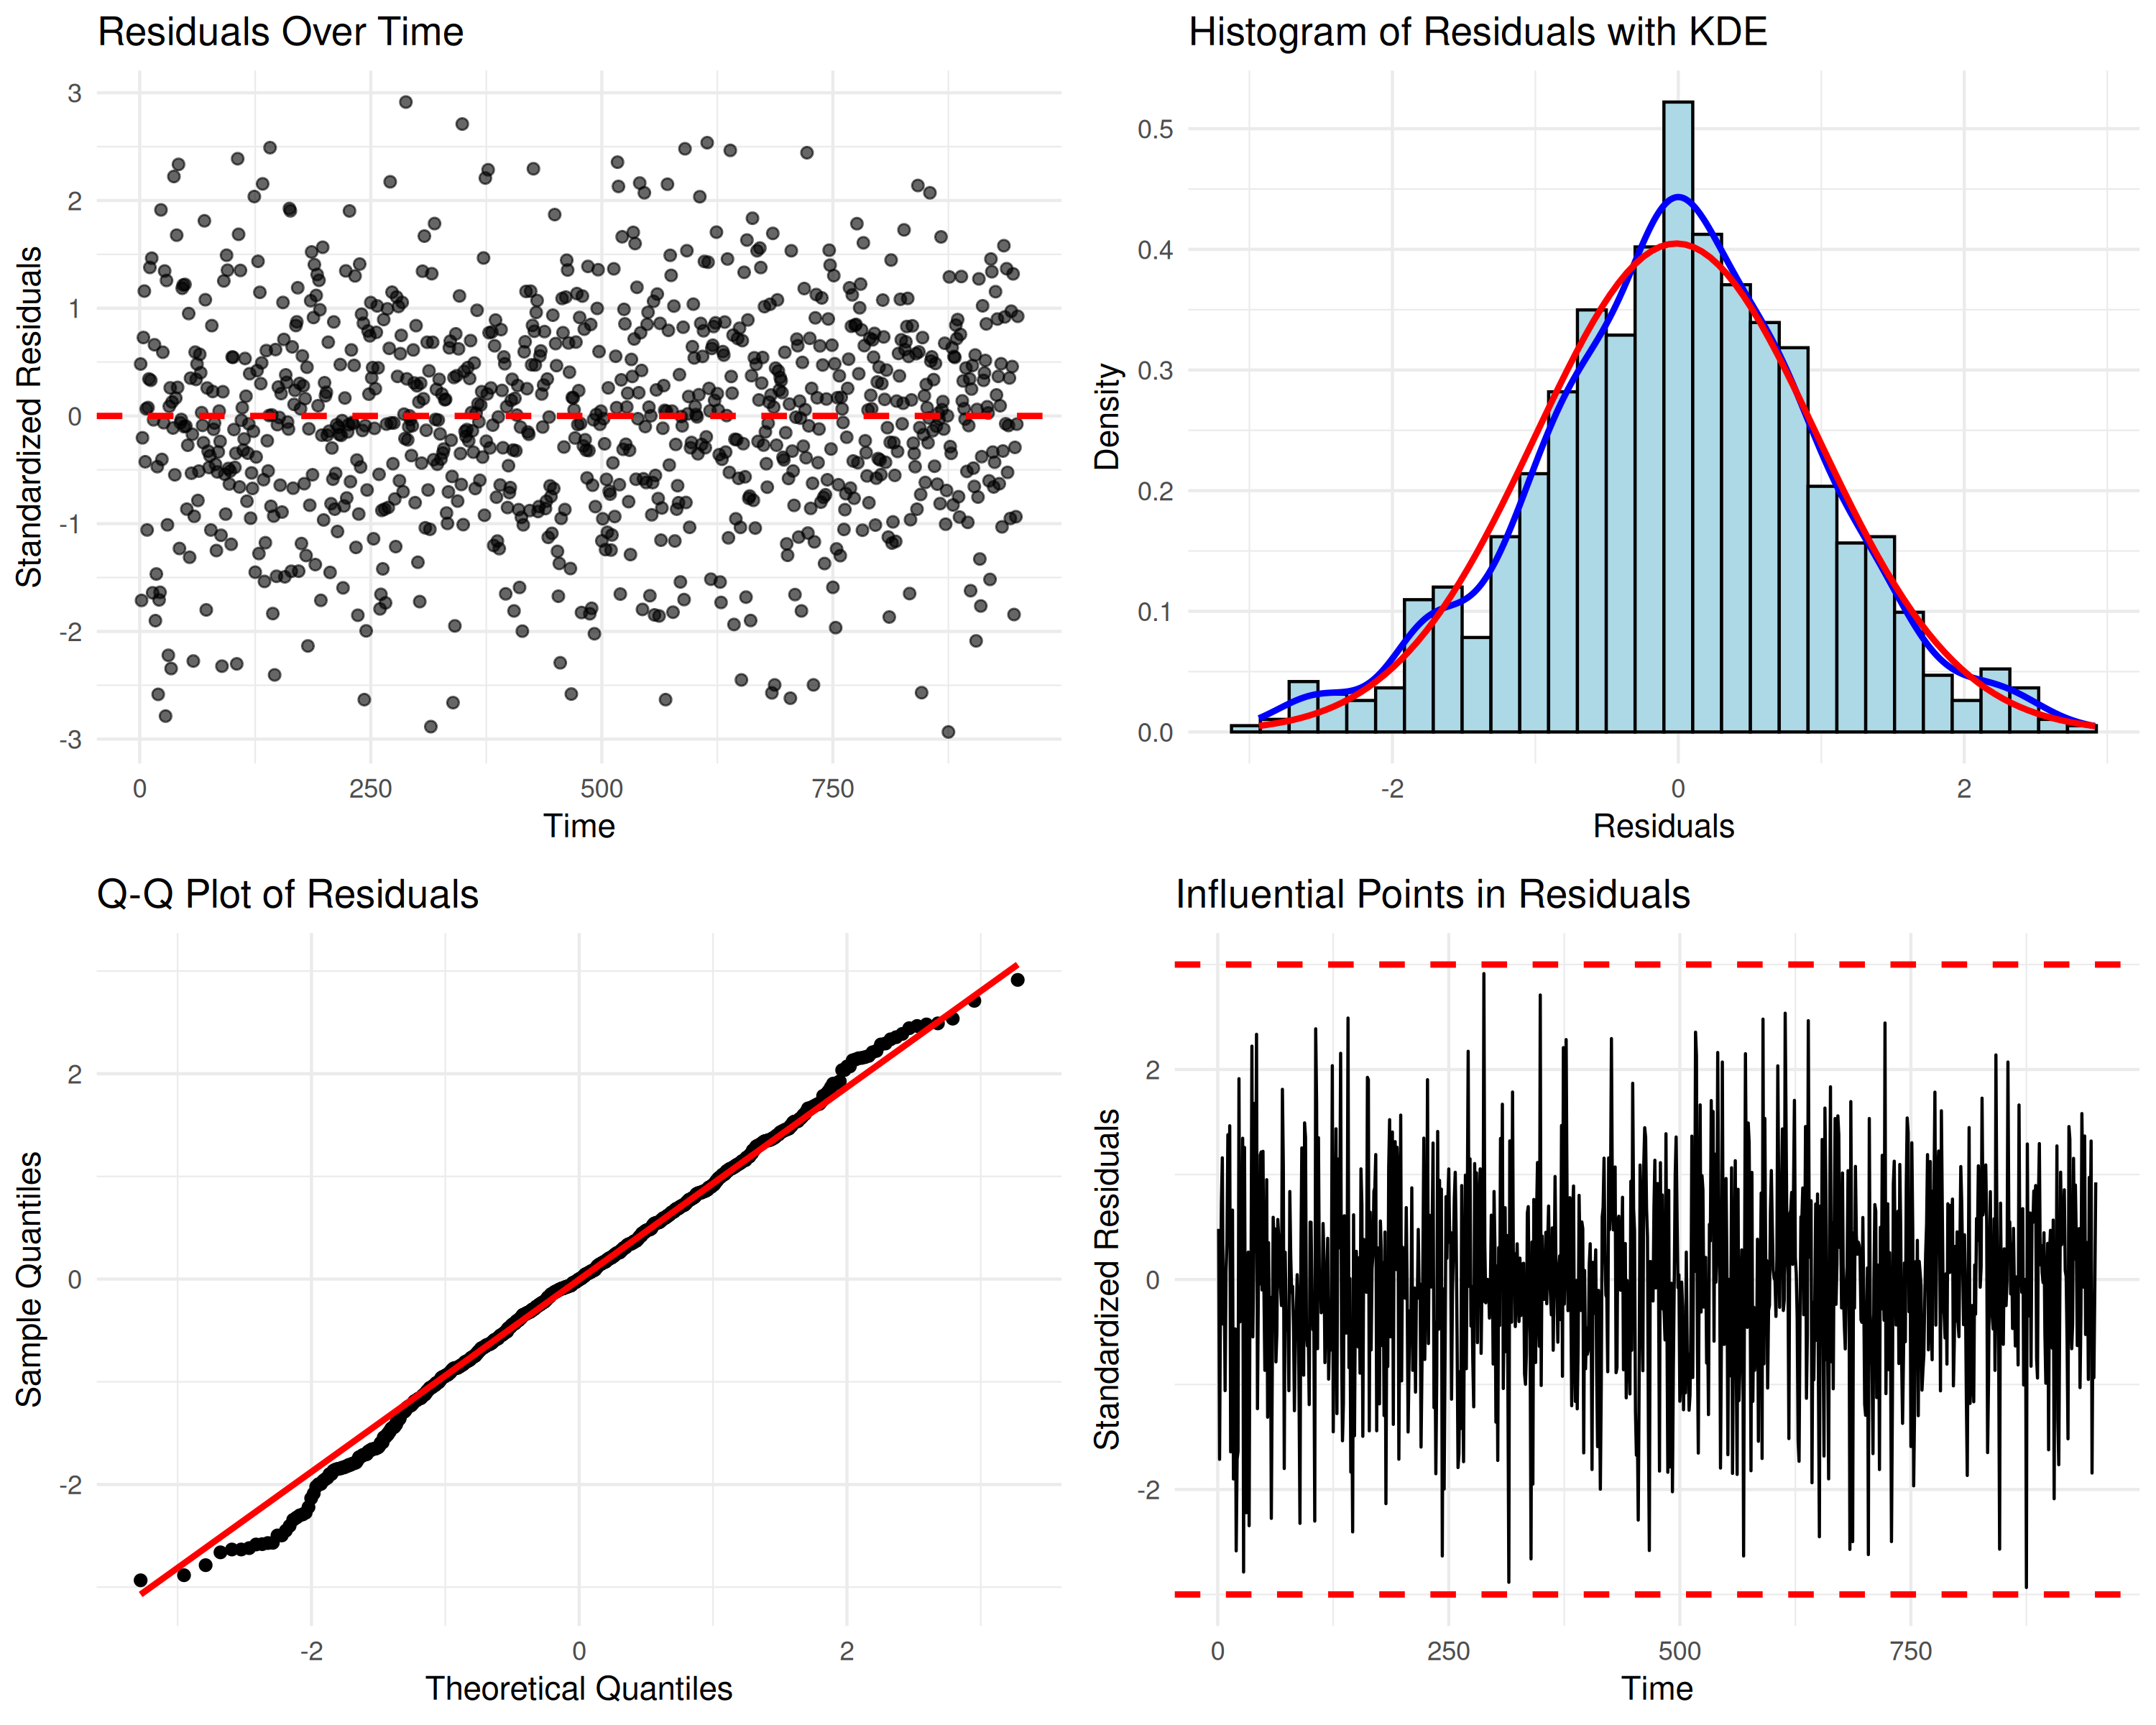
\includegraphics[width=0.8\textwidth]{Residual_Diagnostics.png}
\end{subfigure}

\begin{subfigure}{\textwidth}
    \centering
    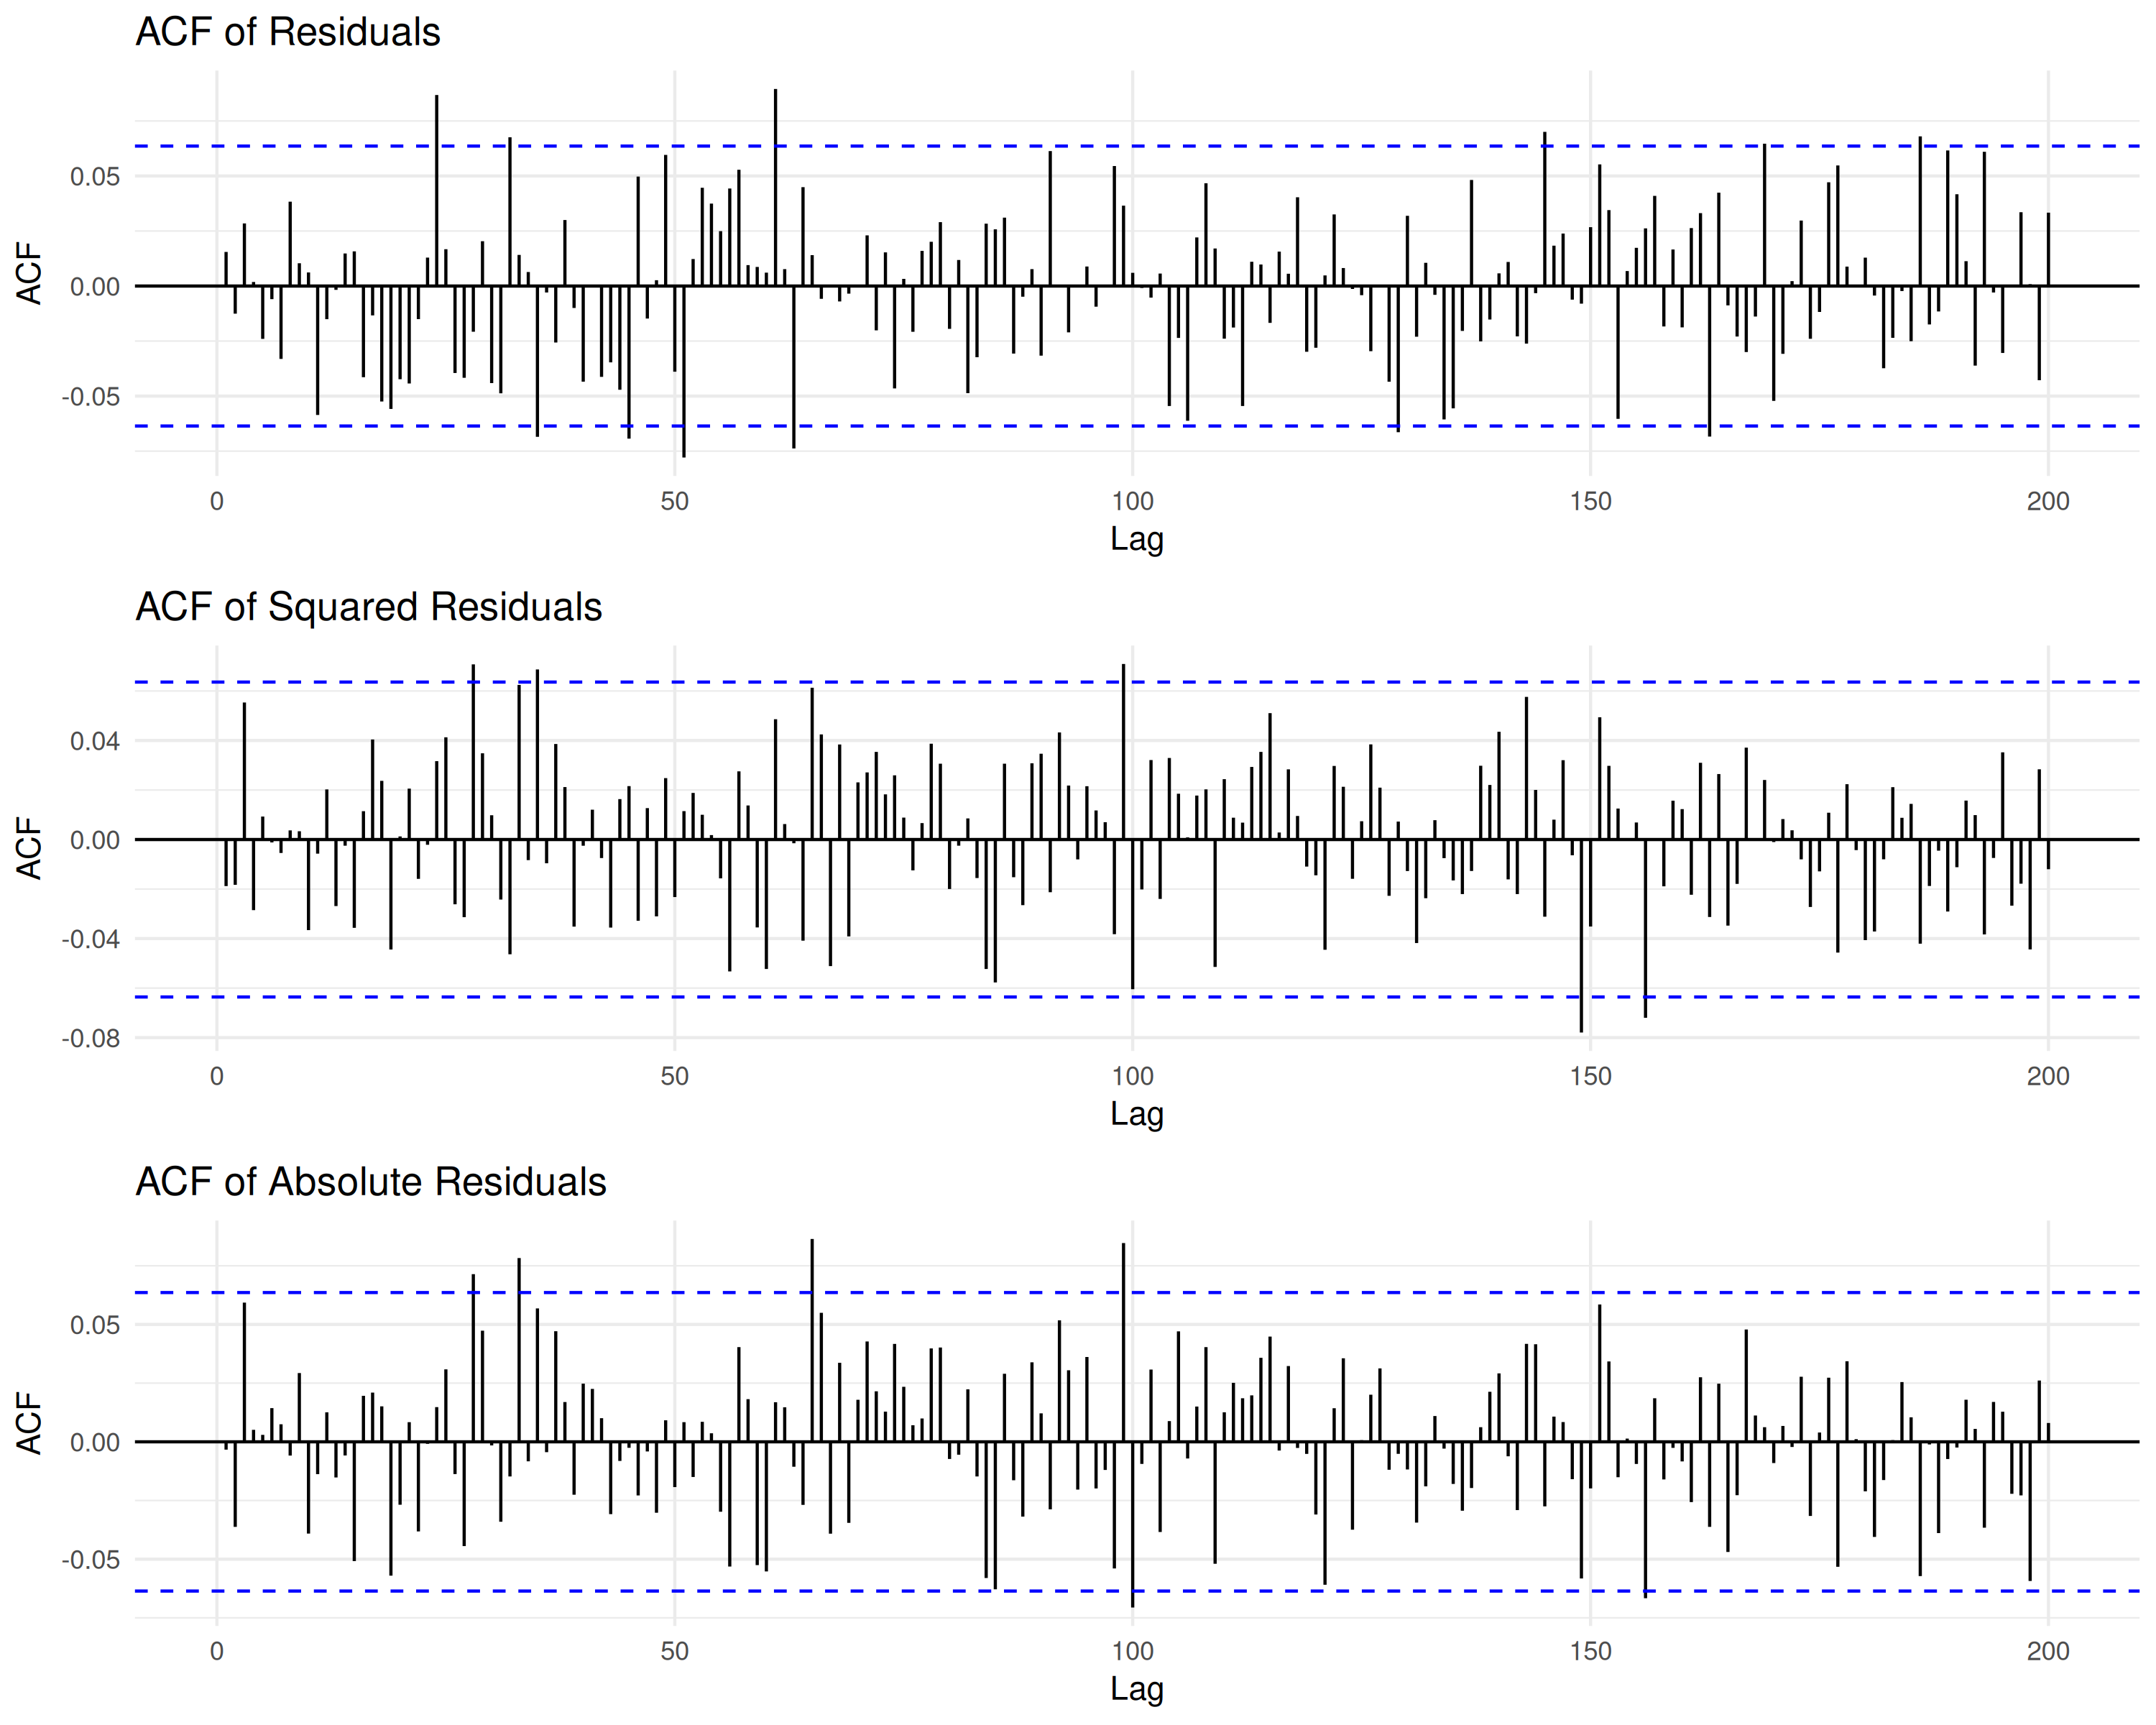
\includegraphics[width=0.75\textwidth]{ACF_plots.png}
\end{subfigure}

\caption{\small{\href{https://github.com/Stochastic1017/Walmart-Stock-Forecasting/blob/main/R/Plot_Residual_Diagnostics.R}{Residual diagnostics for the $\texttt{ARIMA(0,0,1)} + \texttt{GARCH(1,1)}$ model.}}}
\label{fig:residual_diagnostics}
\end{figure}










\section{10-Day Forecast}

\begin{figure}[H]
\centering
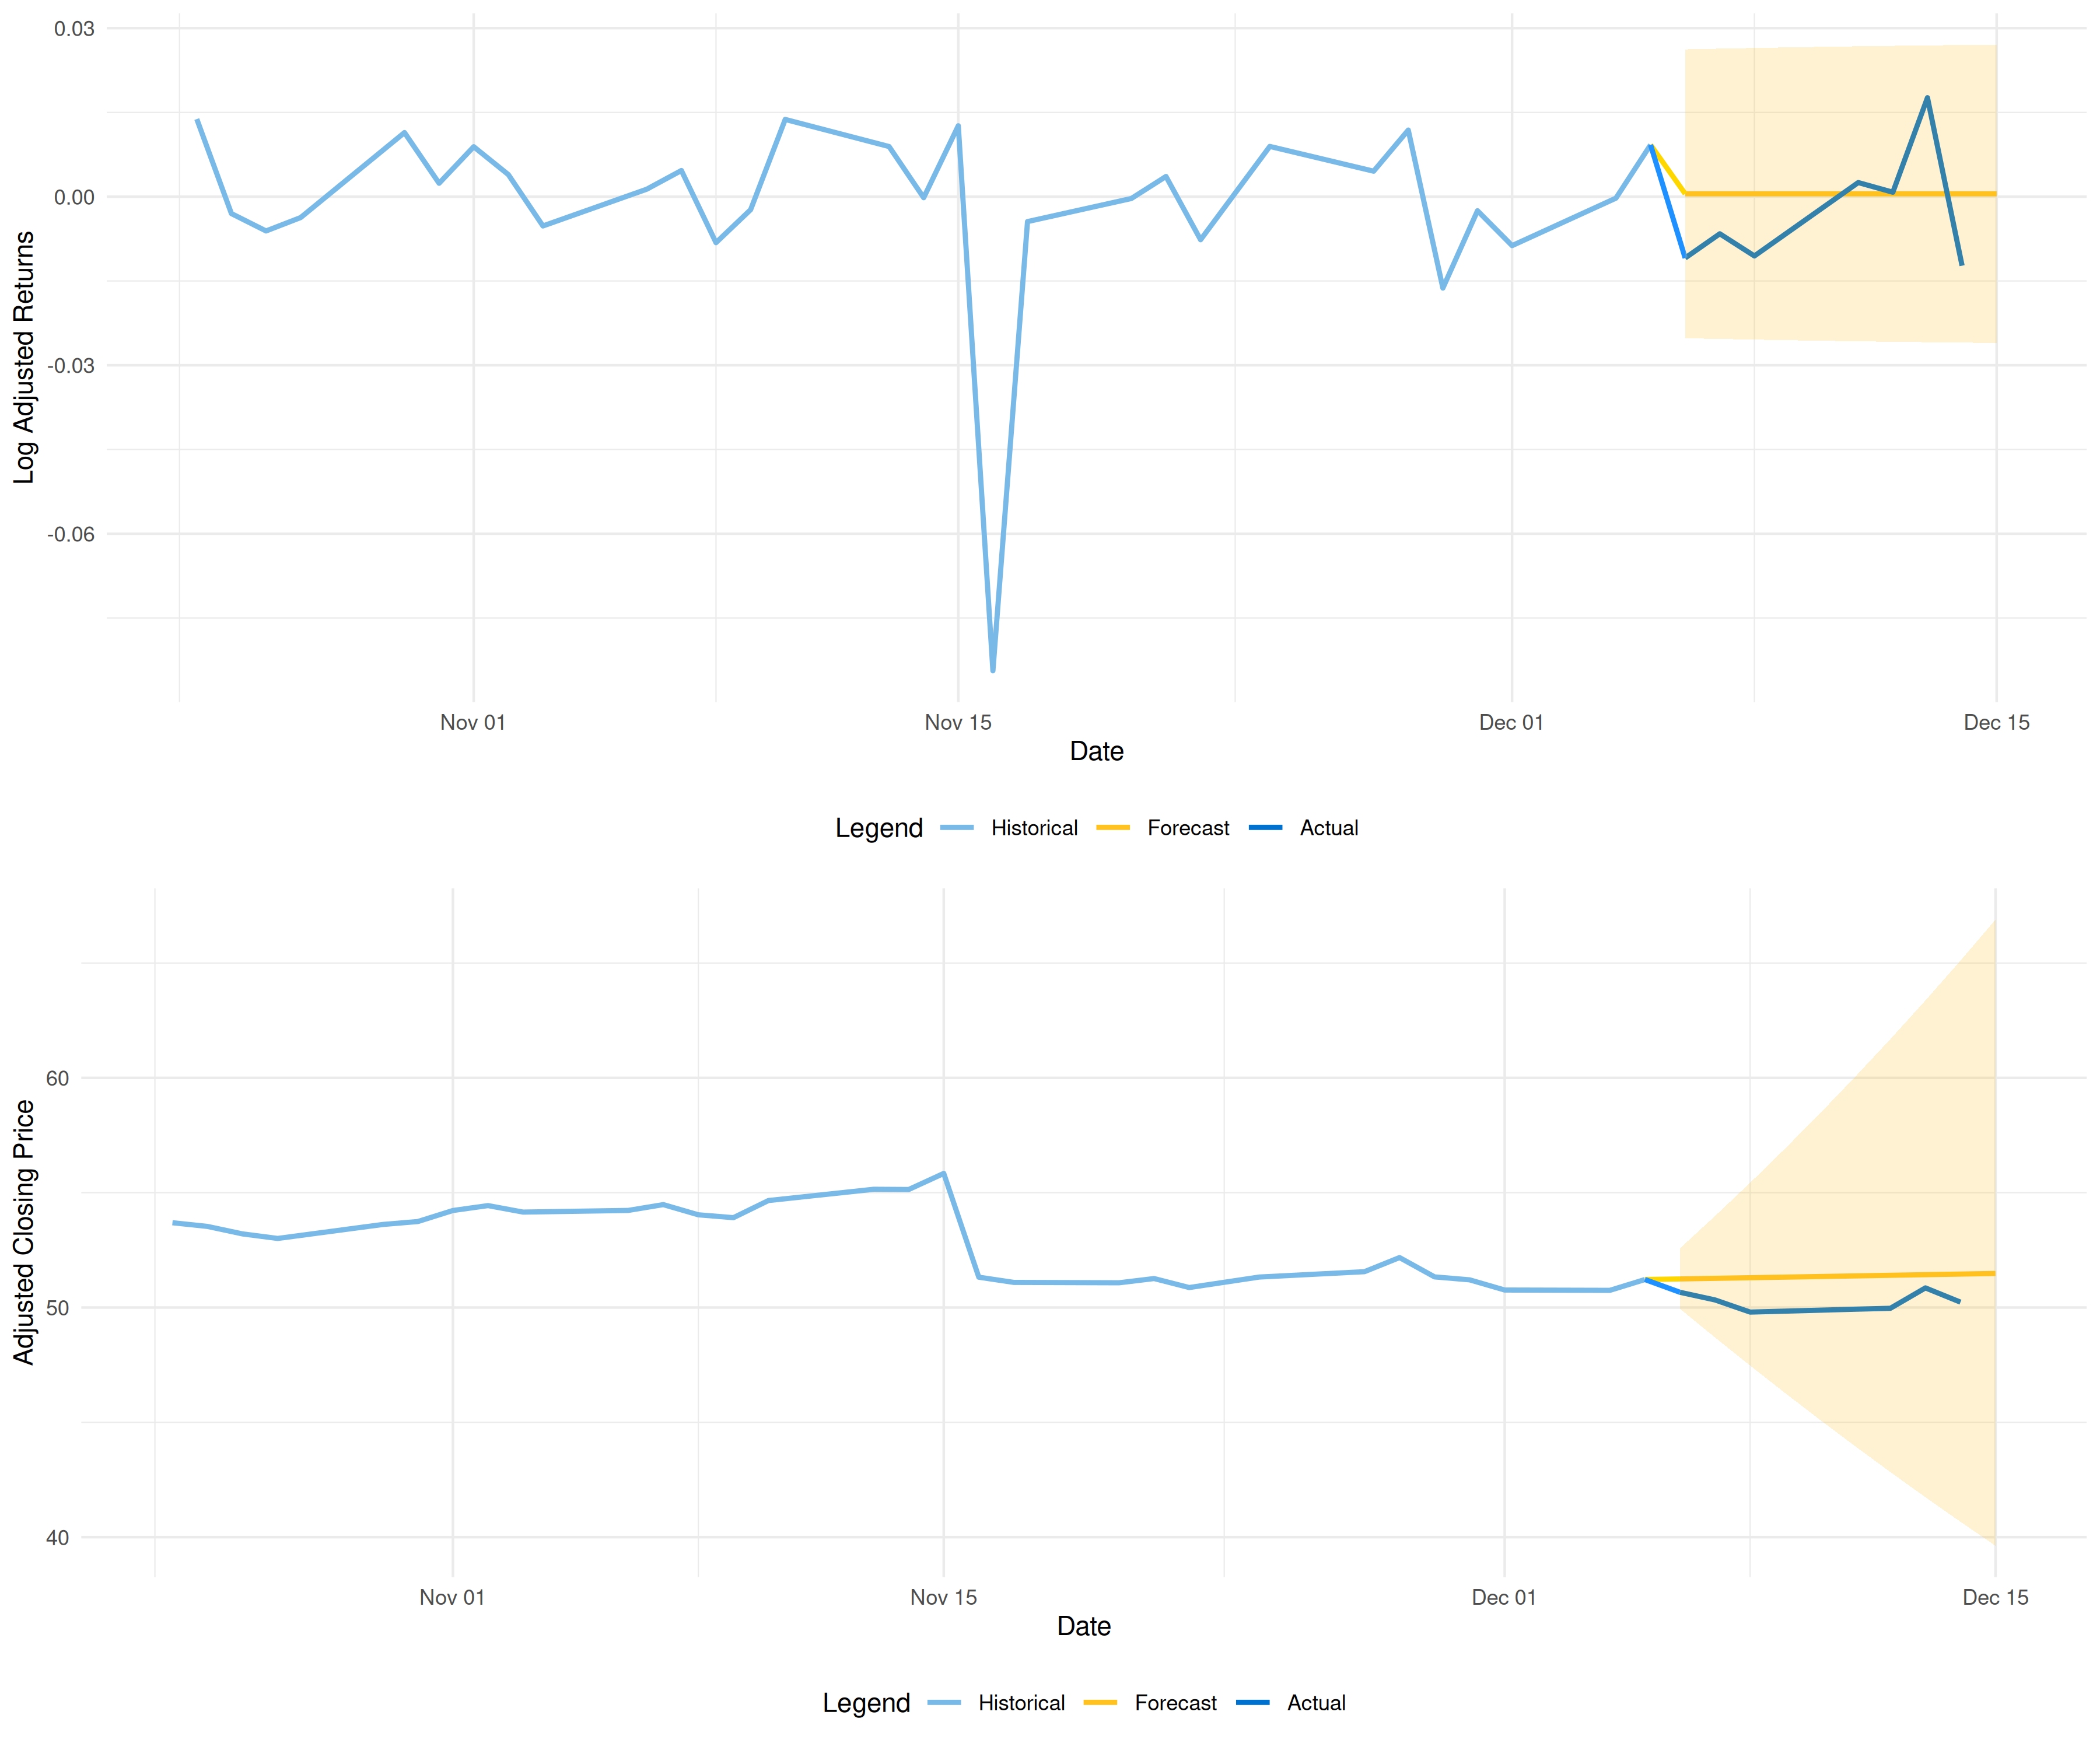
\includegraphics[width=1.0\textwidth]{Forecast.png}
\caption{\small{\href{https://github.com/Stochastic1017/Walmart-Stock-Forecasting/blob/main/R/Plot_Forecast.R}{10-day forecast for log returns and adjusted closing prices, including 95\% confidence intervals, alongside historical and actual data for comparison. (last 30+10 days only). Blue represents historical data, yellow indicates the forecast, and dark blue corresponds to actual observed values.}}}
\label{fig:forecast}
\end{figure}

Figure \ref{fig:forecast} allows us to compare our 10-day forecast with the true log returns and adjusted closing price. It is crucial to note that the model only fits data from \texttt{2020-01-01} to \texttt{2023-12-05}. The actual log returns from \texttt{2023-12-06} to \texttt{2023-12-15} is used to compare model performance on unseen data.

The forecasted log returns align well with the actual values, with all observations falling within the 95\% confidence interval. This indicates that the $\texttt{ARIMA(0,0,1)} + \texttt{GARCH(1,1)}$ model effectively captures the short-term dynamics of the stock. However, the increasing width of the confidence interval for closing prices reflects the compounding effect of forecast uncertainty over time. The RMSE for the 10-day forecast, actual log returns, and adjusted prices were \$ 0.0103 and \$ 1.1693, respectively.

Given the residual diagnostics in Figure \ref{fig:residual_diagnostics} affirmation that the $\texttt{ARIMA(0,0,1)} + \texttt{GARCH(1,1)}$ model effectively captures the underlying structure of Walmart's stock returns, we can conclude that this is a good and effective model for forecasting.



\newpage
\section*{Appendix}

All codes and images associated with this project can be found in the GitHub repository below:

\begin{center}
\url{https://github.com/Stochastic1017/Walmart-Stock-Forecasting}
\end{center}

\textit{Note: The repository will be made public only after \textbf{December 17, 2024 (11:59 PM)} to ensure academic integrity by preventing public access to these materials before the due date.}\\

\begin{table}[H]
\centering
\begin{tabular}{l|r}
\hline
\textbf{Figure/Table}  & \textbf{Code} \\
\hline
Figure \ref{fig:adjclose_adjreturns_plot} & \href{https://github.com/Stochastic1017/Walmart-Stock-Forecasting/blob/main/R/Plot_AdjClose_LogReturns.R}{Code for Figure \ref{fig:adjclose_adjreturns_plot}} \\
Table \ref{tab:arma_model_summary} & \href{https://github.com/Stochastic1017/Walmart-Stock-Forecasting/blob/main/R/Fit_ARMA.R}{Code for Table \ref{tab:arma_model_summary}} \\
Table \ref{tab:arch_garch_model_summary} & \href{https://github.com/Stochastic1017/Walmart-Stock-Forecasting/blob/main/R/Fit_ARCH_GARCH.R}{Code for Table \ref{tab:arch_garch_model_summary}} \\
Table \ref{tab:arma_garch_model_summary} & \href{https://github.com/Stochastic1017/Walmart-Stock-Forecasting/blob/main/R/Fit_ARMA_and_GARCH.R}{Code for Table \ref{tab:arma_garch_model_summary}} \\
Figure \ref{fig:residual_diagnostics} & \href{https://github.com/Stochastic1017/Walmart-Stock-Forecasting/blob/main/R/Plot_Residual_Diagnostics.R}{Code for Figure \ref{fig:residual_diagnostics}} \\
Figure \ref{fig:forecast} & \href{https://github.com/Stochastic1017/Walmart-Stock-Forecasting/blob/main/R/Plot_Forecast.R}{Code for Figure \ref{fig:forecast}} \\
\hline
\end{tabular}
\end{table}

For a more comprehensive analysis and access to all the code used in this project, the following files are available in the repository. Note that each file exceeds the 5-page limit and consolidates all R code used for this project:

\begin{table}[H]
\centering
\begin{tabular}{l|r}
\hline
\textbf{File}  & \textbf{URL} \\
\hline
\texttt{Consolidated-Walmart-Stock-Forecasting.Rmd} & \href{https://github.com/Stochastic1017/Walmart-Stock-Forecasting/blob/main/Rmd/Walmart-Stock-Forecasting.Rmd}{Rmd File Link} \\
\texttt{Consolidated-Walmart-Stock-Forecasting.pdf} & \href{https://github.com/Stochastic1017/Walmart-Stock-Forecasting/blob/main/Rmd/Walmart-Stock-Forecasting.pdf}{PDF File Link} \\
\hline
\end{tabular}
\end{table}

Finally, the LaTeX file and the rendered pdf file associated to this submission write-up is available in this repository:

\begin{table}[H]
\centering
\begin{tabular}{l|r}
\hline
\textbf{File}  & \textbf{URL} \\
\hline
\texttt{Walmart-Stock-Forecasting.tex} & \href{https://github.com/Stochastic1017/Walmart-Stock-Forecasting/blob/main/Rmd/Walmart-Stock-Forecasting.Rmd}{TEX File Link} \\
\texttt{Walmart-Stock-Forecasting.pdf} & \href{https://github.com/Stochastic1017/Walmart-Stock-Forecasting/blob/main/Rmd/Walmart-Stock-Forecasting.pdf}{PDF File Link} \\
\hline
\end{tabular}
\end{table}







\newpage
\section*{Reference}

Bollerslev, T. (1986). Generalized Autoregressive Conditional Heteroskedasticity.
Journal of Econometrics, 31(3), 307–327.

Box G.E.P., Jenkins., G.M., \& Reinsel, G.C. (1994). Time Series Analysis: Forecasting and Control.

Campbell, J.Y., Lo, A.W., \& MacKinlay, A.C. (1997). The Econometrics of Financial Markets.

Diebold, F.X. (2001). Elements of Forecasting.

Engle, R.F. (1982). Autoregressive Conditional Heteroskedasticity with Estimates of the Variance of United Kingdom Inflation. Econometrica, 50(4), 987-1007.

Hansen, P.R., \& Lunde, A. (2005). A Forecast Comparison of Volatility Models: Does Anything Beat a GARCH(1,1). Journal of Applied Econometrics, 20(7), 873-889.

Hamilton, J.D. (1994). Time Series Analysis.

Hyndman, R.J., \& Athanasopoulos, G. (2021). Forecasting: Principles and Practice.

Hull, J.C. (2021). Options, Futures, and Other Derivatives.

Pfaff, B. (2008). Analysis of Integrated and Cointegrated Time Series with R.

Poon, S.H., \& Granger, C.W.J. (2003). Forecasting Volatility in Financial Markets: A Review.
Journal of Economic Literature, 41(2), 478–539.

Tsay, R.S. (2010). Analysis of Financial Time Series.

Zivot, E., \& Wang, J. (2006). Modeling Financial Time Series with S-PLUS.



\end{document}
